

\subsection{Sensor Calibration}

A planar checkerboard pattern was used to calibrate all three cameras to obtain both intrinsic and extrinsic parameters. 
While the grid pattern is not visible in the depth image, it is nevertheless observed in the reflected IR image whose pixels correspond to the depth pixels. 
This enables the use of Zhang's method~\cite{Zhang2000} to calculate the intrinsic parameters including a $2$-parameter radial distortion of each camera. 
In this process the poses of all three cameras are also calculated relative to the checkerboard. 
The intrinsic and extrinsic parameters are stored as text files, and a Matlab function is provided that reads the parameters and can plot the camera poses as in Fig.~\ref{fig:CameraConfiguration}.


\subsubsection{Noise Characterization}
\label{sec:bias}

The time of flight depth measurements can have significant noise, and it is useful to both model it and quantify it. 
Doing so can lead to strategies to reduce noise as well as providing guidance to algorithms that use the depth measurements. 
Our goal in this section is to provide a simple noise model that can predict the empirically observed depth noise on smooth, Lambertian surfaces, such as plant leaves.

The depth noise $\varepsilon$ is modeled as the sum of an image dependent term $\varepsilon_I$ and a sensor dependent term $\varepsilon_S$:
\begin{equation}
\varepsilon = \varepsilon_I + \varepsilon_S. \label{eq:epsilon}
\end{equation}
The term $\varepsilon_I$ is a random variable for each pixel with a value that varies between subsequent images taken from a fixed pose of a static scene.  
On the other hand, $\varepsilon_S$ is a random variable for each pixel that models its depth offset, and its value only changes when the scene changes.  
The variance of $\varepsilon_I$ is estimated for each pixel of a fixed scene observed over multiple images. 
In our experiments we observed a flat, uniform albedo surface perpendicular to the camera at a sequence of depths, and for each depth acquired $300$ images. 
Object depth, $d$, has a large impact on $\varepsilon_I$. 
For constant depth, we observed that the primary factor affecting the variance is the pixel radius $r$, from the image center. 
Physically we expect this dependence is due to a circularly symmetric illuminating beam closely aligned with the optical axis. 
Based on these observations we model $\sigma_I(d,r)$, the standard deviation of $\varepsilon_I$, as a function of depth and pixel radius.  
From our experiments we build up a lookup table for this as plotted in Fig.~\ref{fig:Noise}.

\begin{table*}[t!]
\begin{center}
\caption{Summary of Arabidopsis and Bean databases.\todo{last column needs to be updated}}
\label{tab:stat}
\begin{tabular}{c|c|c|c|c|c}
\hline
% after \\: \hline or \cline{col1-col2} \cline{col3-col4} ...
Plants & Subjects & Days & Images/Day & Total Images & Annotated Images \\
\hline
Arabidopsis & $16$ & $9$ & $16$ & $2304\times 4$ & $576\times 4$ \\
\hline
Bean & $5$ & $5$ & $14$ & $350\times 4$ & $175\times 4$ \\
\hline
\end{tabular}
\end{center}
\end{table*}



\begin{table*}
\begin{center}
\caption{Plant image resolution of Arabidopsis and Bean databases, computed based on the yellow ROIs in Fig.~\ref{fig:fourmodality}.}
\label{tab:resolution}
\begin{tabular}{c|c|c|c|c}
\hline
% after \\: \hline or \cline{col1-col2} \cline{col3-col4} ...
Plants & fluorescence & IR & RGB & depth \\
\hline
Arabidopsis & $\sim$$240\times240$ & $\sim$$240\times240$ & $\sim$$120\times120$ & $\sim$$25\times25$ \\
%\hline
Bean & $1000\times640$ & $1000\times640$ & $380\times720$ & $90\times190$ \\
\hline
\end{tabular}
\end{center}
\end{table*}

Averaging over repeated images of a scene will not remove all the depth error as there are pixel depth offsets that are constant for images of the same scene. 
We model these with $\varepsilon_S$. 
To estimate its standard deviation $\sigma_S$, we first average over many depth measurement images, in our case $300$, to obtain pixel depth estimates that approximately eliminate the effect of $\varepsilon_I$. Then by calculating true ray depths on a known surface, in our case the observed plane, and further assuming that $\varepsilon_S$ has the same standard deviation for all pixels, $\sigma_S$ is obtained as the standard deviation of the error between averaged depths and known depths. In our experiments we obtained $\sigma_S=6.5mm$ and found that it was insensitive to changes in depth.

The recorded depth images in the data collection are the result of averaging $N=5$ subsequent depth images.  
Assuming independence of $\varepsilon_I$ and $\varepsilon_S$, the variance of pixel depth measurements is given by:
\begin{equation}
\sigma^2(d,r) = \frac{\sigma_I^2(d,r)}{N} + \sigma_S^2.\label{eq:sigma}
\end{equation}

There are additional sources of noise not modeled by this.  
Object albedo has an impact although this is fairly weak for strong signal reflections.  
Factors with large impact on signal noise include: object specularities, sharp variations in object albedo, mixed-depth pixels on object edges, and cases of very-low signal reflection, all of which can lead to very large variances. 
One of the utilities of having a model for variance is that it can be compared with the measured variance, and the difference used as a cue for portions of the scene that violate our modeling assumptions.

In addition, we noticed that the chamber light shades blocked some of the depth camera field of view, and in doing so reflected some of the IR illumination. 
This resulted in a small constant depth shift for the pixels. 
We measured this shift for each chamber experiment and provide it as an optional correction to the depth images.

%\begin{figure}
%\begin{centering}
%\begin{tabular}{c }
%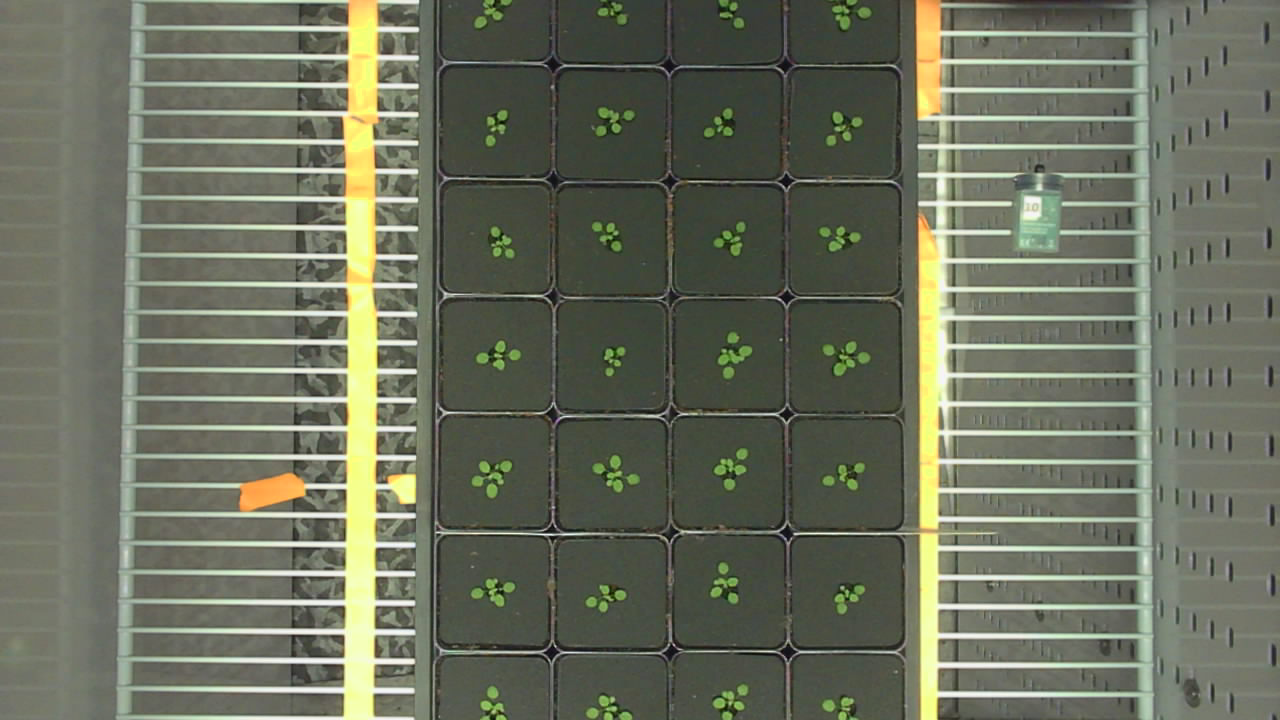
\includegraphics[width=.47\textwidth]{Figures/rawImages/a.png}\\
%Arabidopsis \\
%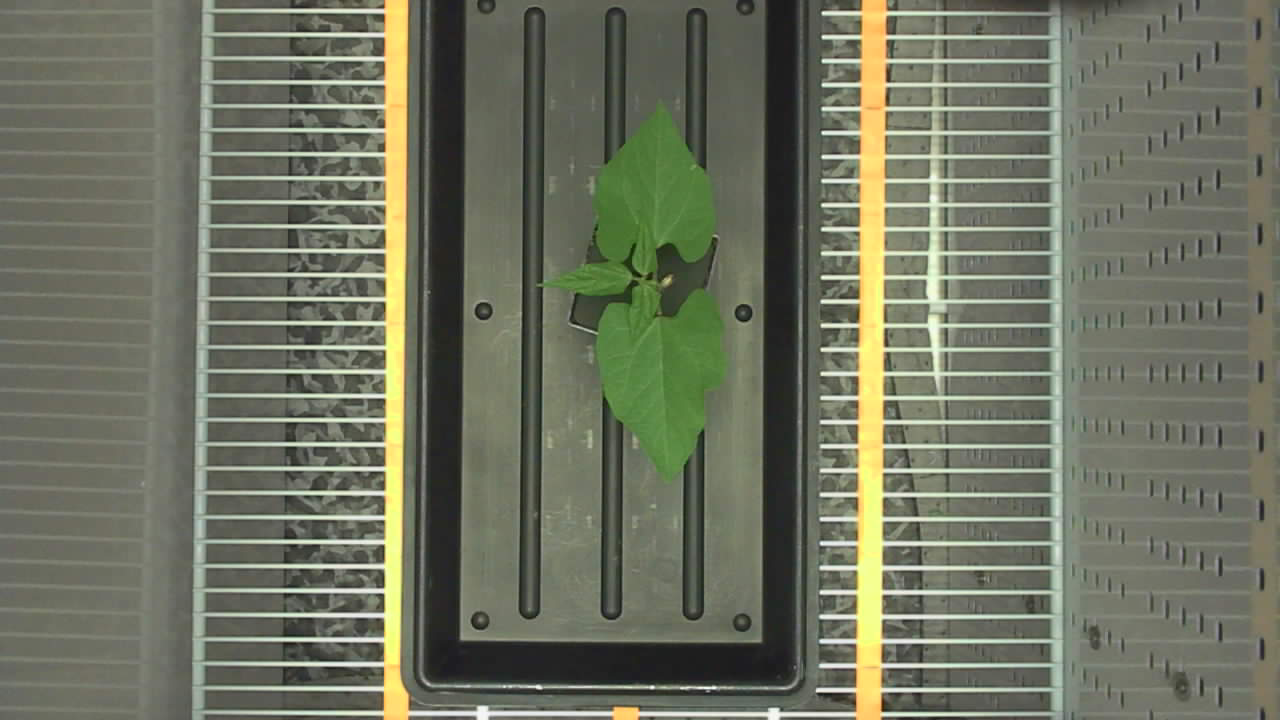
\includegraphics[width=.47\textwidth]{Figures/rawImages/b.png}\\
% Bean \\
%\end{tabular}
%\caption{RGB color images of Arabidopsis and bean plants. }
%\label{fig:rawIm}
%\end{centering}
%\end{figure}





